\section{Preliminaries}

In order to ensure the security of a software system, not only is it important to design a robust security architecture (intended) but it also is necessary to preserve the security of the  (implemented) architecture during software evolution as presented in \cite{alferez2014dynamic}. Therefore, security knowledge is usually presented as reusable techniques to help engineers and developers designing, implementing and maintaining secure systems. Some of these approaches are, for instance, defensive programming, design security patterns and design by contracts. This section  introduces the last two approaches as they constitute the basis of the contract-based security pattern approach presented in this paper.

\subsection{Security design patterns}

In software engineering, a design pattern is a general, reusable solution to a commonly occurring problem within a given software design context. It is not a finished design that can be transformed directly into source or machine code. It rather is a description or template for how to solve a problem that can be used in many different situations.

A design pattern is classically composed of three parts:
\begin{itemize}
    \item The \emph{problem}. This part describes in a few sentences which problem is addressed by the pattern.
    
    \item The \emph{solution}. This part is usually composed of a UML (Unified Modeling Language) class diagram and a few sentences to explain the diagram.

    \item The \emph{remarks}. The authors of the pattern can add in this part any information they think is relevant. It usually involves performance results.
\end{itemize}

With the rise of cyber security, new design patterns -- security design patterns -- have been developed to provide generic solutions to fulfill some common security goals such as authentication, authorization and secure message delivery. The following subsection presents the authentication pattern. It is also used throughout this paper to exemplify our approach and implementations.

\subsubsection{Authentication pattern}

The goal of this pattern is to verify the identity of a subject. Such a subject can be someone interacting with a software by providing credentials, a subsystem requesting data to another subsystem, a thread requesting extra privilege to an operating system, etc. The pattern only provides an architecture which is compatible with the use of every authentication algorithm. The architecture of the Authentication pattern is presented in Figure \ref{fig:my_label}.

\begin{figure}
    \centering
    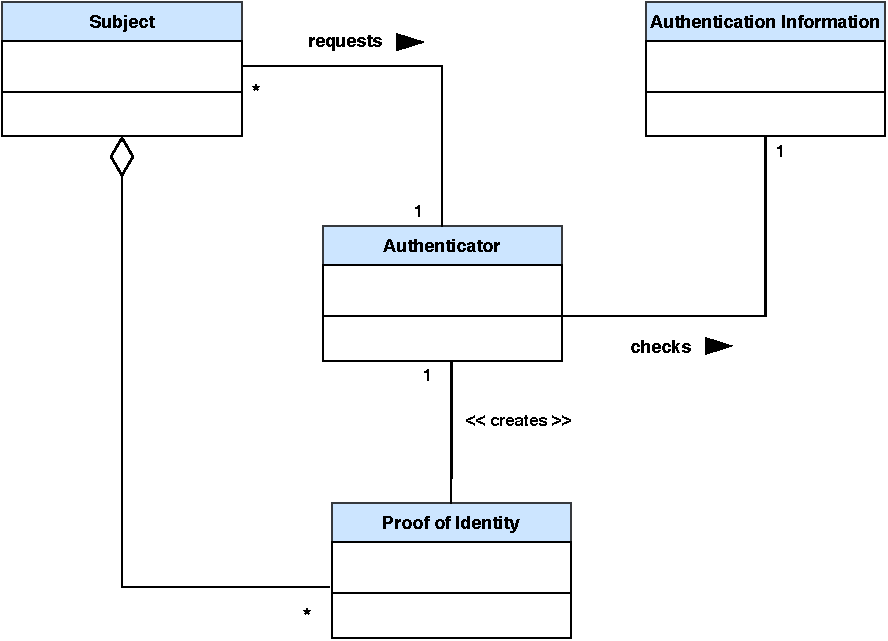
\includegraphics[width=1\columnwidth]{utils/authenticator_CD.pdf}
    \caption{UML class diagram of the Authentication pattern}
    \label{fig:my_label}
\end{figure}

It is composed of four parts:
\begin{itemize}
    \item a \textit{Subject} needing to be authenticated,
    \item a \textit{Proof of Identity}, token given to the subject once the authentication is complete,
    \item an \textit{Authenticator} is the object which implements an authentication algorithm and creates the \textit{Proof of Identity},
    \item \textit{Authentication Information} are the information provided by the \textit{Subject} to the \textit{Authenticator}.

\end{itemize}

%This pattern provides a solution which implicitly separates the \textit{Authenticator} entity from the \textit{Authentication Information}. This type of architecture although more complex is still preferred because it is harder to compromise such a system: an attacker would have to compromise both the \textit{Authenticator} and the \textit{Authentication Information} database to gain access to their expected \textit{Proof of Identity}.

% Sylvain: Expliquer ici que dans le cadre d'une mise en oeuvre de ce pattern, les différents "acteurs" du pattern sont soit des composants déjà existants, soit des composants à aller chercher, soit des composants auxquels fournir des points d'extension, soit des composants à développer, etc... Sinon évidemment on utiliserait des bibliothèques de trucs déjà tout prêts.
%Est-ce que ces détails sont nécessaires pour la suite?

%\subsubsection{Authorization pattern}

%The goal of the Authorization pattern is to identify a subject requesting a resource and to be able to check whether the subject is authorized or not to access it. Once again, the exact nature of the subject and the resource are not defined in the pattern and can be pretty much anything (client and database, user and file access privilege, etc.).

%\begin{figure}
%    \centering
%    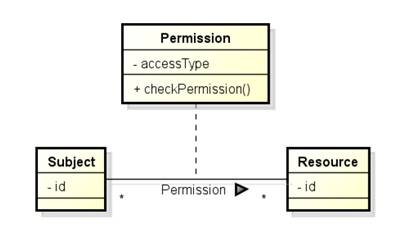
\includegraphics{utils/authorization_CD.png}
%    \caption{UML class diagram of the Authorization pattern}
%    \label{fig:my_label}
%\end{figure}

%This architecture is composed of three entities:
%\begin{itemize}
%    \item the \textit{Subject}, which requires access to a \textit{Resource},
%    \item the \textit{Resource} represents what the \textit{Subject} is allowed to access,
%    \item the \textit{Permission}, which represents one way to access the \textit{Resource} and encapsulates a mechanism to check the validity of the access.
%\end{itemize}

%For this pattern to be relevant, both \textit{Subjects} and \textit{Resources} must be identified in a relevant way: two subjects with the same identifier cannot have different privileges. One way to ensure this property is to give different identifiers to every \textit{Subject} and every \textit{Resource}.
%what does "to be relevant" mean? what does "identified in a relevant way" mean?

%\subsubsection{Pattern composition}
%create a link between the two patterns
%A single and isolated security pattern is usually not enough to secure a system. Thus, multiple security patterns are usually used together, in a process called pattern composition, to improve the security of a software system. For instance, scenarios such as the one in which an application needs to know the identity of the current user and after authentication, it needs to authorize access (to certain resources) to some authenticated users, illustrate a composition process of the Authentication and Authorization security patterns.
% Sylvain: Parler ici de la composition de ces patterns. Mettre en évidence qu'un même composant logiciel peut jour un rôle dans un pattern, et un autre rôle dans un autre pattern

\subsubsection{Limitations of design patterns}\label{PatternLimitations}

The use of design patterns has many advantages for software development as they bring a certain uniformity in software design. They provide a common language between software designers and developers and make software more easily maintainable and extensible. As a generic solution, the definition of a design pattern is usually abstracted from the implementation. Although this abstraction allows for pattern reusability, it is problematic when it comes to security. Indeed, most attacks on software systems are based on weaknesses in the implementation, referred to as vulnerabilities. The presence of natural language in the definition of patterns also introduces potential vulnerabilities, as it is subject to interpretation. In particular, the implementation details are usually implied in the security pattern definition. Therefore, the use of security design patterns does not guarantee the security of a software, as their definition is not formal enough, and thus ambiguous.

\subsection{Design by contract}

The Design by Contract (DbC) concept was coined by Meyer \cite{meyer1992applying} as an approach to design reliable software based on the idea that elements of a software system collaborate with each other on the basis of mutual obligations and benefits.

The whole DbC approach relies on the idea of contract. Meyer indeed realized that most of the software systems, and in particular object-oriented systems, depend on the division of work. This means that tasks are classically divided in several sub-tasks, each being conducted by a program unit. 
%This kind of organization can also be observed in most professional situations. 
Most of the time, the completion of a given task is made possible by the division of labor between several actors. When this happens, the actual interaction of the actors is entirely defined in a \emph{contract}. This contract contains the liabilities and benefits of the interaction for all parties involved. This analogy led Meyer to the idea of software contracting \cite{meyer1992applying}: to define contracts between clients (i.e., routine’s callers) and suppliers (i.e., routines, functions or methods).
A contract is defined as the aggregation of two assertions to a routine or method:
\begin{itemize}
    \item A precondition:  Boolean condition that needs to be verified before calling the routine. It summarizes the client's obligations towards the supplier.
    \item A postcondition: Boolean condition that needs to be verified after the call is made. It summarizes the supplier's obligations towards the client.
\end{itemize}

The whole idea of the DbC approach is that since a contract is formally defined for each service (routine or method), bugs are unlikely to appear at run-time because of a misunderstanding between program units.

In addition to these two assertions, Meyer defined a third type of Boolean expression called a \textit{class invariant}. This notion relies on the class concept. In object-oriented designs, a class should be the representation of some specific concept, usually referred to as object or model. Most of the time, a few properties characterize the essence of the class and should be true at all time and for every instance. A classic example of this idea is the binary tree node class in which all nodes are connected to at most two nodes. A node instance of such a structure should verify at any time that both its children reference it as their respective parent node. This property is then an \textit{Invariant} for this class.